\setlength{\columnsep}{3pt}
\begin{flushleft}

\begin{itemize}
	\item RAM stands for \textbf{R}andom \textbf{A}ccess \textbf{M}emory.
	\item Usage of RAM:
	\begin{itemize}
		\item CPU uses RAM as \textbf{short term memory} for data storage.
		\item Used by computer to store actively used data for quick access.
	\end{itemize}
	\item How much RAM is recommended according to usage?
	\begin{itemize}
		\item \textbf{6GB - 8GB} - Normal usage and internet browsing.
		\item \textbf{16GB} - For spreadsheets and other office programs.
		\item \textbf{32GB} or more - For gamers and multimedia creators.
		\item \textbf{64GB} \& more - For servers.
	\end{itemize}

	\begin{figure}[h!]
		\centering
		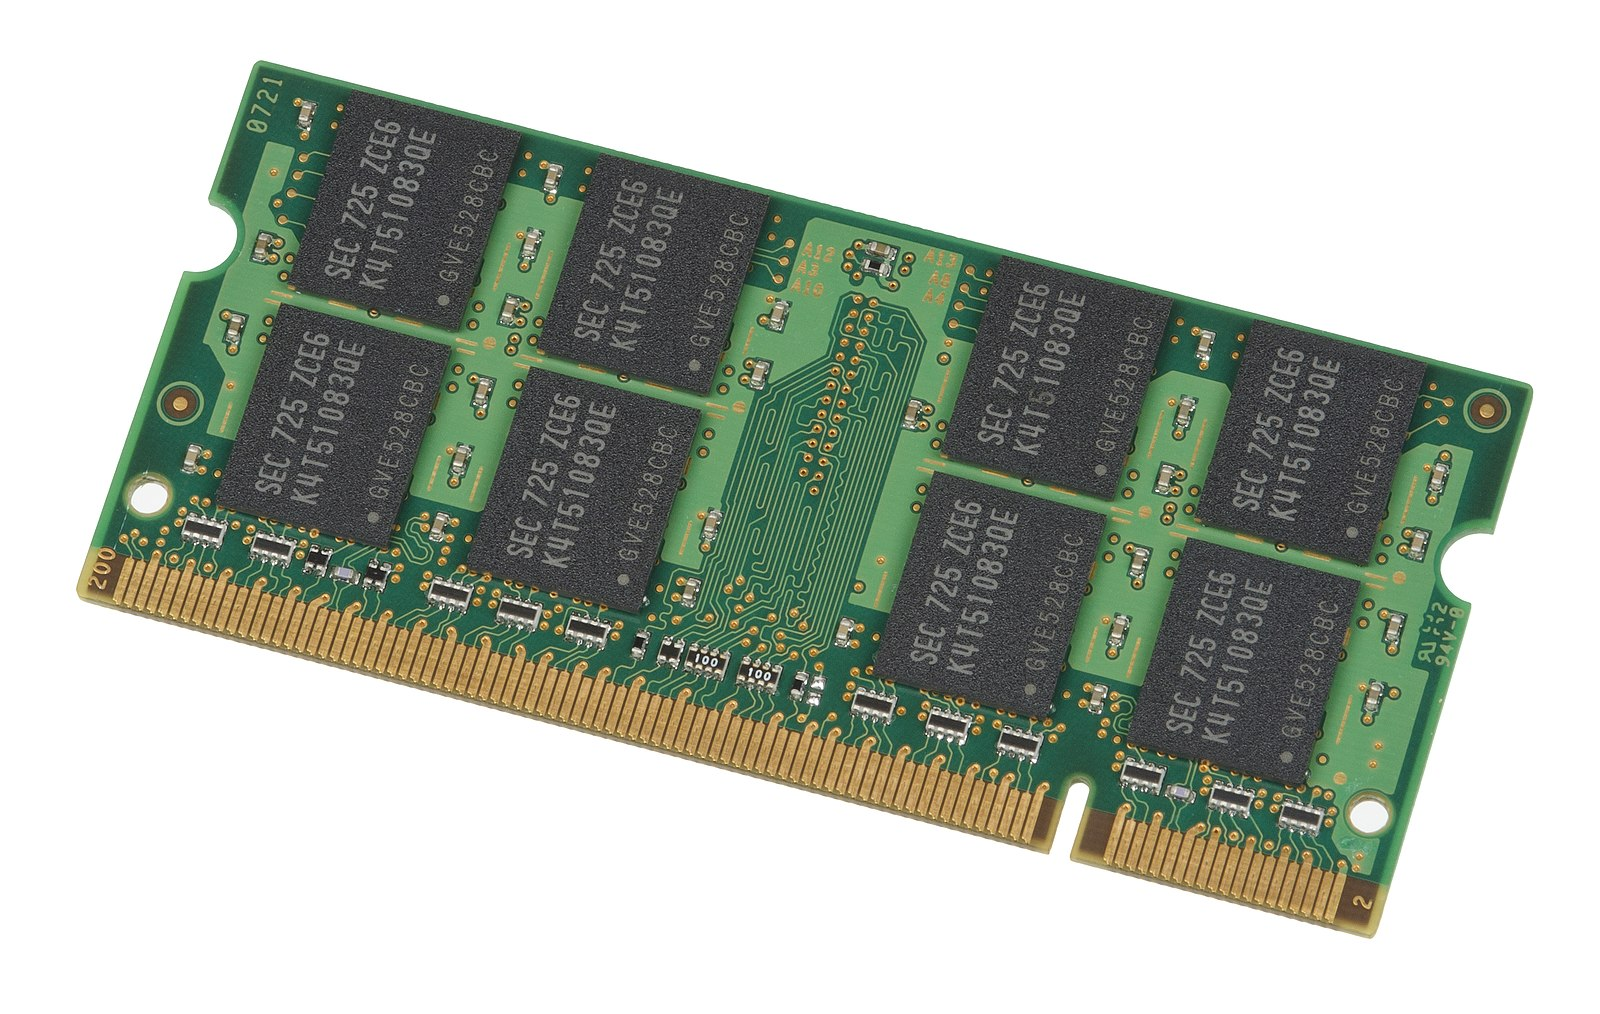
\includegraphics[scale=.15]{content/chapter12/images/ram.jpg}
		\caption{RAM}
		\label{fig:ram}
	\end{figure}

	\item Compared to HDD, RAM is expensive. RAM price according to size:
	\begin{itemize}
			\item 2GB - Approx Rs. 950
			\item 4GB - Approx Rs. 1750
			\item 8GB - Approx Rs. 2940
	\end{itemize}

	\item All memory details are stored in \textbf{/proc/meminfo}.
	\bigskip
	\begin{tcolorbox}[breakable,notitle,boxrule=-0pt,colback=pink,colframe=pink]
		\color{black}
		\fontdimen2\font=1em
		Syntax: less /proc/meminfo
		\fontdimen2\font=4pt
	\end{tcolorbox}



\end{itemize}

\end{flushleft}

\newpage


